%***********************************************************************************************************%
%*************************************FORMATO GENERAL DEL DOCUMENTO*****************************************%
%***********************************************************************************************************%

%Tipo de hoja, tamaño de letra, estilo general:
\documentclass[a4paper,11pt]{article}


%***********************************************************************************************************%
%*****************************************INCLUSIÓN DE PAQUETES*********************************************%
%***********************************************************************************************************%

%Estilos de idioma:
%\usepackage[spanish]{babel}

%Mapea determinados caracteres a macros:
%\usepackage[utf8]{inputenc}

%Gráficos y colores:
\usepackage[pdftex]{graphicx}	% No se puede usar con epsfig
\usepackage{subfig}
\usepackage{graphicx}
\usepackage[usenames,dvipsnames]{color}
\DeclareGraphicsExtensions{.bmp,.png,.jpg,.pdf,.mps,.gif}

%Para poder definir cualquier tamaño de márgenes:
\usepackage{anysize}

%Utilidades para tablas (ej: multicolumn):
\usepackage{array}
%Para poder unir filas en las tablas
\usepackage{multirow}
%Para añadir colores a las tablas:
\usepackage{colortbl}
%Para poder ajustar el ancho de tablas de forma automática:
\usepackage{booktabs}
\usepackage{tabulary}

%Utilizar fuentes bbm en entornos matemáticos:
\usepackage{bbm}

%Características adicionales para escribir fórmulas matemáticas:
\usepackage{amsmath}
\usepackage{amssymb}
\usepackage{amsfonts}

%Para poder crear XYmatrix (p.ej., diagramas de bloques):
\usepackage[all]{xy}

%Estilos de cuadros (línea simple, sombreado, etc.):
\usepackage{fancybox}

%Reimplementar los comandos \setcounter, \addtocounter, \setlength, and \addtolength. Ahora aceptan cualquier tipo de expresión como parámetro, no sólo valores fijos:
\usepackage{calc}

%Personalización de encabezado y pie de página:
\usepackage{fancyhdr}

%Para poder usar la opción 'H' en el posicionado de figuras:
\usepackage{float}

%Requerido para poder usar laprint:
%\usepackage{psfrag}

%Para poder incluir figuras en formato eps:
%\usepackage{epsfig}

%Para poder dibujar figuras arbitrarias con comandos:
%\usepackage{pstricks}  %   Nota: Impide incluir archivos en pdf. Por eso hay que usar el paquete epsfig.
                       %   Para compilar: ALT+2, ALT+4, ALT+8

%Para poder dibujar circuitos eléctricos y electrónicos:
%\usepackage{pst-circ}

%Para poder insertar código (MatLab, C, ...) con formato adecuado:
\usepackage{listings}

%Para insertar hipervínculos:
\usepackage[pdftex]{hyperref}

%Para poder insertar el símbolo del euro (\euro):
\usepackage{eurosym}



%***********************************************************************************************************%
%****************************************PROPIEDADES DEL FICHERO********************************************%
%***********************************************************************************************************%

%Espaciado:
\frenchspacing

%Tamaño de márgenes:
\marginsize{3cm}{2.5cm}{2cm}{2cm}   % Controla los márgenes {izquierda}{derecha}{arriba}{abajo}

%Encabezado y pie de página:
%\pagestyle{fancy}
%\setlength{\headheight}{15.8pt} % Porque el tamaño por defecto del encabezado es demasiado pequeño
%para este formato
%\fancyhf{}                      % Borra el formato preestablecido para encabezado y pie de página
%\fancyhead[RO]{\leftmark}       % En las páginas impares (O), parte derecha del encabezado (R),
%aparecerá el capítulo
%\fancyhead[LO]{\includegraphics[width=0.95cm]{images/MHPLogo.png}}
%\fancyhead[RO]{TRATAMIENTO DIGITAL DE IMÁGENES (2009/2010)}
%\fancyhead[LO]{\textcolor{blue}{RROO}}
%\fancyhead[RE]{\rightmark}      % En las páginas pares (E), parte derecha del encabezado (R), aparecerá el nombre de sección
%\fancyhead[RO,LE]{\thepage}     % Números de página en las esquinas de los encabezados
%\fancyhead[RO,LE]{\thepage}     % Números de página en las esquinas de los encabezados
%\fancyfoot[CO]{\thepage}        % Número de página en el pie de las páginas impares (O) y centrado
%(C)
%\renewcommand{\footrulewidth}{0.4pt} % Si se pone agrega también una línea en el pie de página

%Definición de funciones matemáticas:
\def\prodd{\displaystyle\prod}
\def\sumd{\displaystyle\sum}
\def\intd{\displaystyle\int}
\def\limd{\displaystyle\lim}

%***********************************************************************************************************%
%****************************PROPIEDADES DE LISTINGS (PARA CÓDIGO EN MATLAB)********************************%
%***********************************************************************************************************%

%Definimos el color de fondo:
\definecolor{ColorFondo}{rgb}{0.96,0.96,0.96}

%Propiedades de listings:
\lstloadlanguages{matlab}
\lstset{  frame=Ltb,
     framerule=0pt,
     aboveskip=0.5cm,
     framextopmargin=3pt,
     framexbottommargin=3pt,
     framexleftmargin=0.4cm,
     framesep=0pt,
     rulesep=.4pt,
     backgroundcolor=\color{ColorFondo},
     rulesepcolor=\color{black},
     %
     stringstyle=\ttfamily,
     showstringspaces = false,
     basicstyle=\small\ttfamily,
     commentstyle=\color{green},
     keywordstyle=\bfseries,
     %
     numbers=left,
     numbersep=15pt,
     numberstyle=\tiny,
     numberfirstline = false,
     breaklines=true,
     %
}

%Para minimizar fragmentado de listados:
\lstnewenvironment{listing}[1][]
   {\lstset{#1}\pagebreak[0]}{\pagebreak[0]}
\lstdefinestyle{Matlab}
   {language=matlab,
    emph={function,for,end,if,else,elseif,clear,close,while,switch,case,otherwise},
    % Lista de comandos que se quieren enfatizar
    emphstyle=\color{blue},
    basicstyle=\scriptsize,
    commentstyle=\color[rgb]{0.133,0.545,0.133},
    stringstyle=\color[rgb]{0.627,0.126,0.941},
    morekeywords={besselj,char,imread,imshow,makecform,applycform,imnoise,medfilt2,fspecial,
                  imfilter,uint8,double,imhist,cat,logical,im2double,strel,imerode,imdilate,
                  im2bw,rgb2ycbcr,ycbcr2rgb,plot3,regionprops,imcrop,ones,xcorr,repmat},
                  % Lista de comandos adicionales que se quieren resaltar
   }


%***********************************************************************************************************%
%****************************************PROPIEDADES DE HYPERREF********************************************%
%***********************************************************************************************************%

\hypersetup{
%    bookmarks=true,         % show bookmarks bar?
    unicode=false,          % non-Latin characters in Acrobat’s bookmarks
    pdftoolbar=true,        % show Acrobat’s toolbar?
    pdfmenubar=true,        % show Acrobat’s menu?
    pdffitwindow=false,     % window fit to page when opened
    pdfstartview={FitH},    % fits the width of the page to the window
    pdftitle={Tarea},% title
    pdfkeywords={keywords}, % list of keywords
    pdfnewwindow=true,      % links in new window
    colorlinks=true,        % false: boxed links; true: colored links
    linkcolor=black,        % color of internal links
    citecolor=red,          % color of links to bibliography
    filecolor=magenta,      % color of file links
    urlcolor=blue           % color of external links
    %plainpages=false,       % 
}


%***********************************************************************************************************%
%*************************************************NOTAS*****************************************************%
%***********************************************************************************************************%

% -Para incluir un fichero o un código en Matlab:
%      \lstinputlisting[style=Matlab]{fichero.m}
%     o bien:
%      \begin{lstlisting}[style=Matlab] código \end{lstlisting}
% -Para usar laprint (requiere incluir el paquete psfrag), en MatLab hay que escribir:
%     set(0,'defaulttextinterpreter','none');
%     laprint;
% -Para incluir un fichero .tex:
%     \input{fichero.tex}
%

%\begin{figure}
% \centering
%  \subfloat[One.]{\includegraphics[width=0.3\textwidth]{images/Convertidas/Mejora/2-1Recortada.png}}
%  \hspace{.25in}
%  \subfloat[Two.]{\includegraphics[width=0.15\textwidth]{images/Convertidas/Mejora/2-1Recortada.png}}
%  \subfloat[Two.]{\includegraphics[width=0.15\textwidth]{images/Convertidas/Mejora/2-1Recortada.png}} \\
%  \subfloat[Three.]{\includegraphics[width=0.3\textwidth]{images/Convertidas/Mejora/2-1Recortada.png}}
%  \hspace{.25in}
%  \subfloat[Four.]{\includegraphics[width=0.3\textwidth]{images/Convertidas/Mejora/2-1Recortada.png}}
%  \caption{Simple Case.}
%\end{figure}


%***********************************************************************************************************%
%************************************************OPENING****************************************************%
%***********************************************************************************************************%

%Definimos el color del título:
\definecolor{ColorTitulo}{rgb}{0,0.08,0.3}
\definecolor{ColorSubTitulo}{rgb}{0.05,0.12,0.9}
\definecolor{ColorFecha}{rgb}{0.25,0.25,0.4}

%Título, autores y fecha:
\title{\Huge{\textcolor{ColorTitulo}{\textbf{Multiuser Channel Estimation:\\Simulation Results}} \\}}
\author{}
\date{}


%***********************************************************************************************************%
%**************************************PARTE INICIAL DEL DOCUMENTO******************************************%
%***********************************************************************************************************%

\begin{document}

% \pagenumbering{alph}
% 
\maketitle %\thispagestyle{empty}
% 
% \newpage
% 
% \clearpage\pagenumbering{roman}
% 
% \tableofcontents
% 
% \newpage



%***********************************************************************************************************%
%***********************************************DOCUMENTO***************************************************%
%***********************************************************************************************************%

% \newpage
% 
% \clearpage\pagenumbering{arabic}

\section{Comparison FFBS and PGAS}

\begin{figure}[H]
\centering
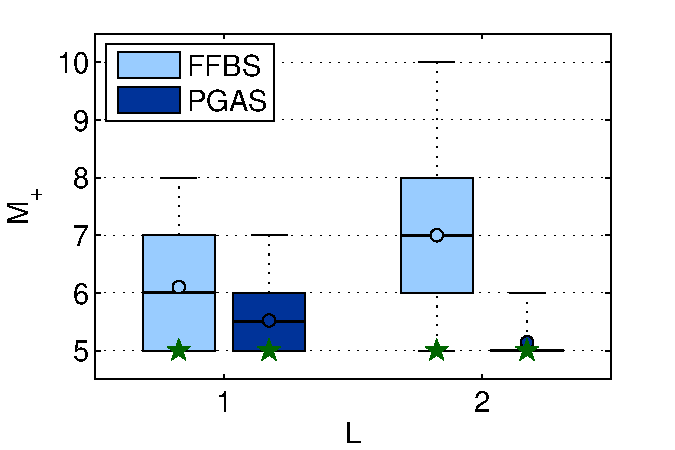
\includegraphics[width=.3\textwidth]{ffbs_pgas/ffbs_pgas.pdf}
\caption{Inferred number of transmitters for FFBS and PGAS methods.}\label{fig:ffbs_pgas}
\end{figure}

\section{Simulation Results}

Differences with respect to EUSIPCO simulations: (i) Observation period $T=1000$ instead of $500$, and (ii) burst length of $500$ time instants, instead of being random with mean value $250$.

% SNR
\begin{figure}[H]
\centering
\subfloat[Inferred $\hat{M}_+$.]{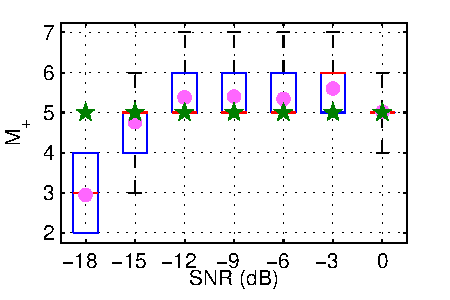
\includegraphics[width=.25\textwidth]{L1/BoxM_SNR_s.pdf}}
\subfloat[ADER.]{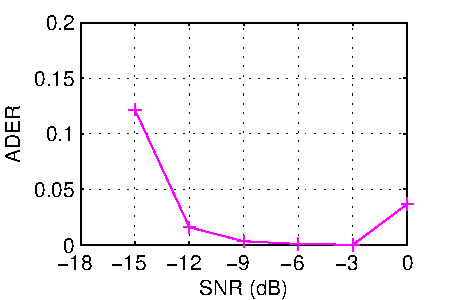
\includegraphics[width=.25\textwidth]{L1/ADER_SNR_s.pdf}}
\subfloat[SER.]{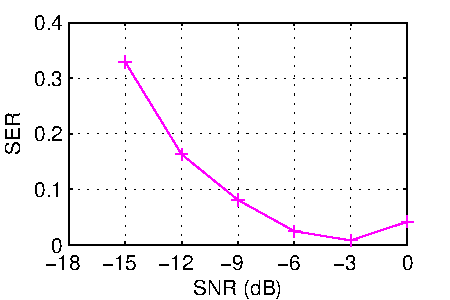
\includegraphics[width=.25\textwidth]{L1/SER_SNR_s.pdf}}
\subfloat[MSE.]{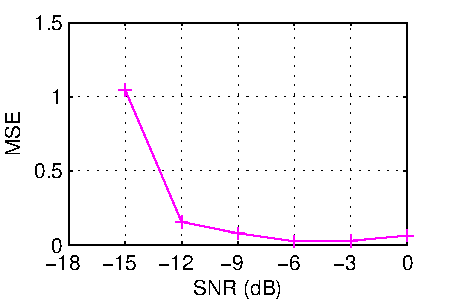
\includegraphics[width=.25\textwidth]{L1/MSE_SNR_s.pdf}}
\caption{Results for different SRNs ($L=1$).}\label{fig:resultsSNR_L1}
\end{figure}

\begin{figure}[H]
\centering
\subfloat[Inferred $\hat{M}_+$.]{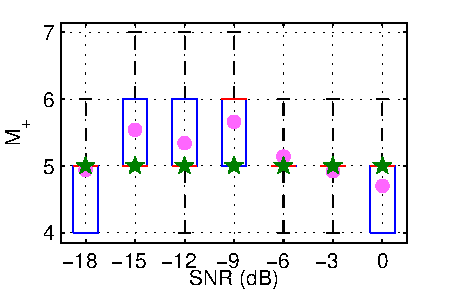
\includegraphics[width=.25\textwidth]{L3/BoxM_SNR_s.pdf}}
\subfloat[ADER.]{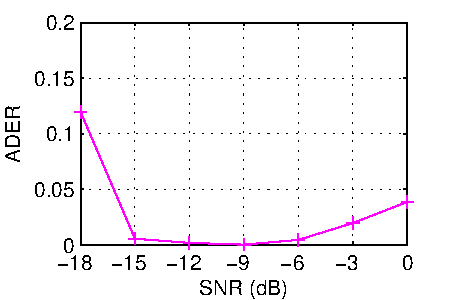
\includegraphics[width=.25\textwidth]{L3/ADER_SNR_s.pdf}}
\subfloat[SER.]{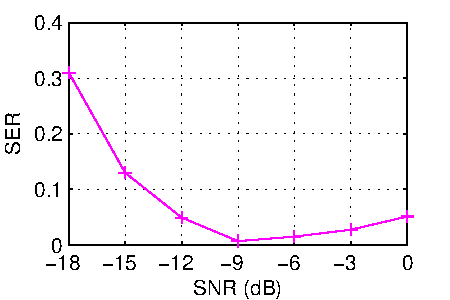
\includegraphics[width=.25\textwidth]{L3/SER_SNR_s.pdf}}
\subfloat[MSE.]{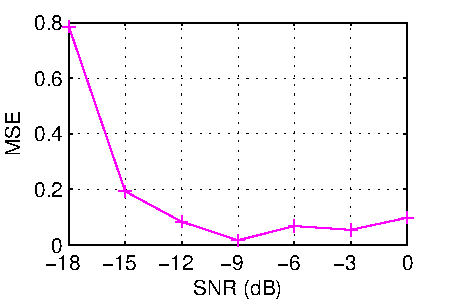
\includegraphics[width=.25\textwidth]{L3/MSE_SNR_s.pdf}}
\caption{Results for different SRNs ($L=3$).}\label{fig:resultsSNR_L3}
\end{figure}

% Nt
\begin{figure}[H]
\centering
\subfloat[Inferred $\hat{M}_+$.]{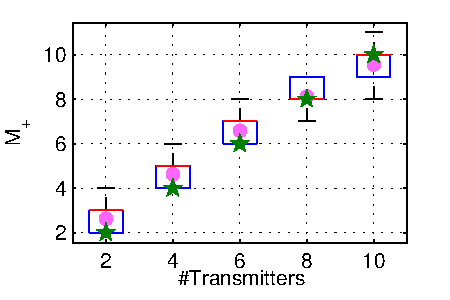
\includegraphics[width=.25\textwidth]{L1/BoxM_Nt_s.pdf}}
\subfloat[ADER.]{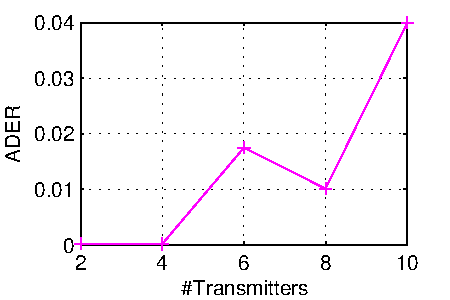
\includegraphics[width=.25\textwidth]{L1/ADER_Nt_s.pdf}}
\subfloat[SER.]{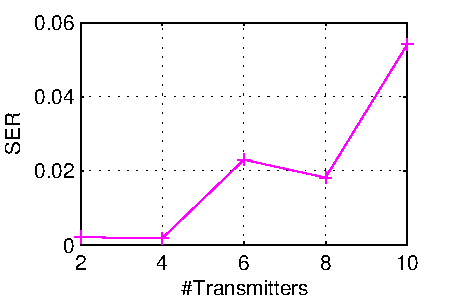
\includegraphics[width=.25\textwidth]{L1/SER_Nt_s.pdf}}
\subfloat[MSE.]{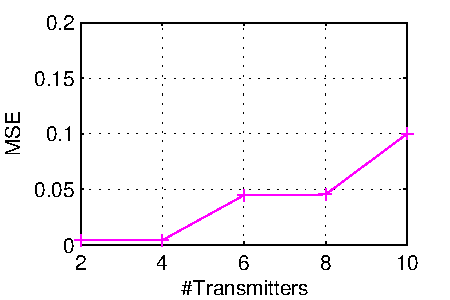
\includegraphics[width=.25\textwidth]{L1/MSE_Nt_s.pdf}}
\caption{Results for different number of transmitters ($L=1$).}\label{fig:resultsNt_L1}
\end{figure}

\begin{figure}[H]
\centering
\subfloat[Inferred $\hat{M}_+$.]{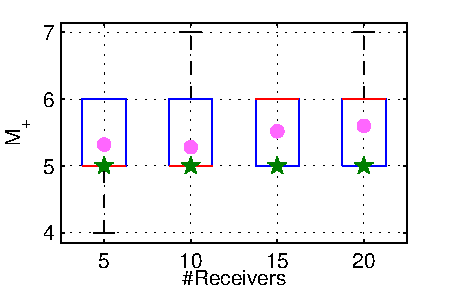
\includegraphics[width=.25\textwidth]{L1/BoxM_Nr_s.pdf}}
\subfloat[ADER.]{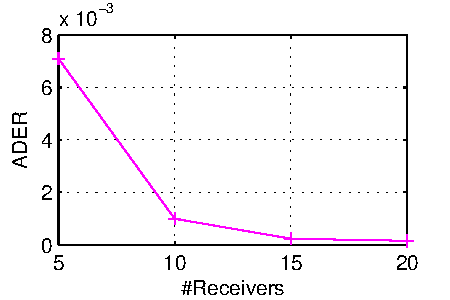
\includegraphics[width=.25\textwidth]{L1/ADER_Nr_s.pdf}}
\subfloat[SER.]{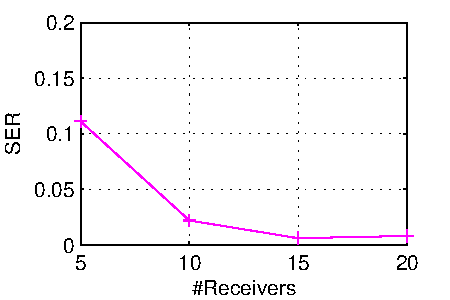
\includegraphics[width=.25\textwidth]{L1/SER_Nr_s.pdf}}
\subfloat[MSE.]{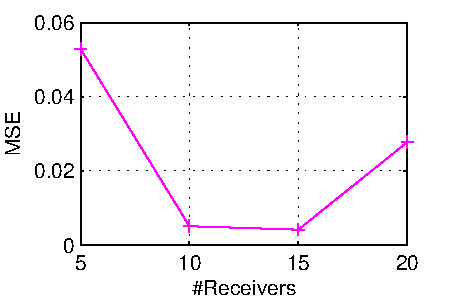
\includegraphics[width=.25\textwidth]{L1/MSE_Nr_s.pdf}}
\caption{Results for different number of receiving antennas ($L=1$).}\label{fig:resultsNr_L1}
\end{figure}

\begin{figure}[H]
\centering
\subfloat[Inferred $\hat{M}_+$.]{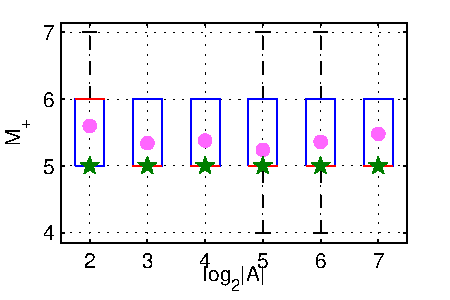
\includegraphics[width=.25\textwidth]{L1/BoxM_M_s.pdf}}
\subfloat[ADER.]{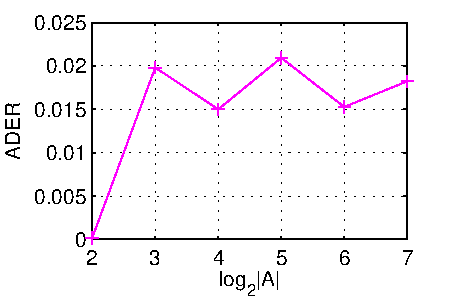
\includegraphics[width=.25\textwidth]{L1/ADER_M_s.pdf}}
\subfloat[SER.]{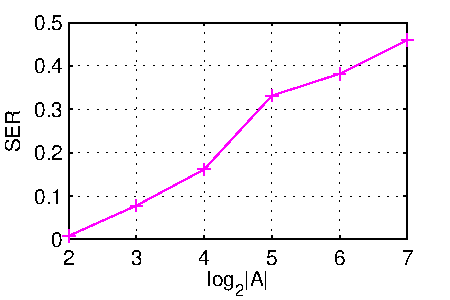
\includegraphics[width=.25\textwidth]{L1/SER_M_s.pdf}}
\subfloat[MSE.]{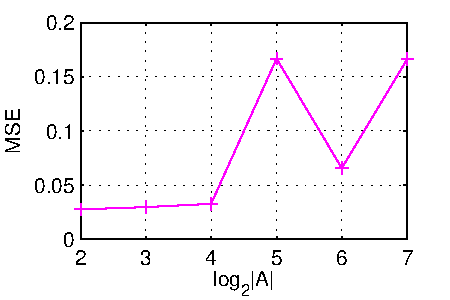
\includegraphics[width=.25\textwidth]{L1/MSE_M_s.pdf}}
\caption{Results for different constellation order ($L=1$).}\label{fig:resultsM_L1}
\end{figure}


\begin{figure}[H]
\centering
\subfloat[Inferred $\hat{M}_+$.]{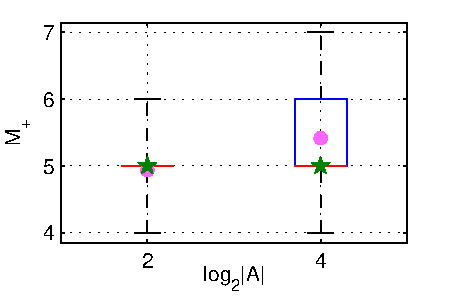
\includegraphics[width=.25\textwidth]{L3/BoxM_M_s.pdf}}
\subfloat[ADER.]{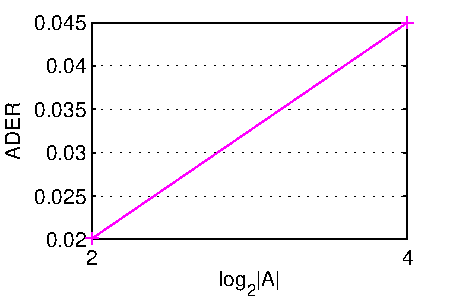
\includegraphics[width=.25\textwidth]{L3/ADER_M_s.pdf}}
\subfloat[SER.]{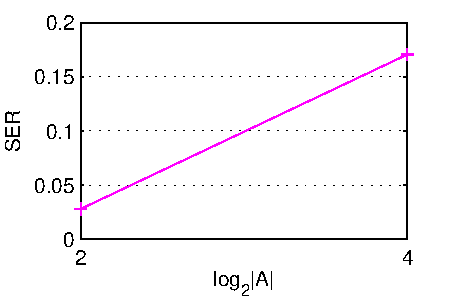
\includegraphics[width=.25\textwidth]{L3/SER_M_s.pdf}}
\subfloat[MSE.]{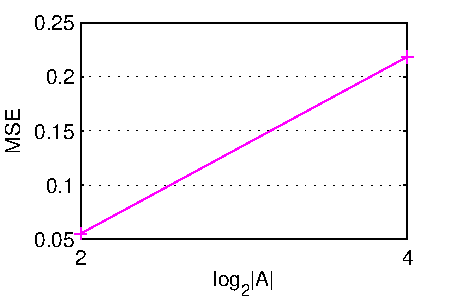
\includegraphics[width=.25\textwidth]{L3/MSE_M_s.pdf}}
\caption{Results for different constellation order ($L=3$).}\label{fig:resultsM_L3}
\end{figure}




%***********************************************************************************************************%
%*******************************************APÉNDICES/ANEXOS************************************************%
%***********************************************************************************************************%



%***********************************************************************************************************%
%*********************************************BIBLIOGRAFÍA**************************************************%
%***********************************************************************************************************%

%Para que se incluyan todos las entradas de los ficheros .bib, aunque no hayan sido citadas
%\nocite{*}
%Inserción de ficheros .bib:
%\bibliography{Bibliografia}{} \addtocounter{page}{62}
% Add entry to table of contents:
%\addcontentsline{toc}{section}{Bibliograf\'{\i}a}
%Estilo de la bibliografía:
%\bibliographystyle{unsrt}


%\begin{thebibliography}{99}
%\end{thebibliography}


\end{document}

